\chapter{SYSTEM ARCHITECTURE} \label{chap_sys_architecture}
System architecture is explained and analyzed under three sub sections.
\begin{enumerate}
    \item Main overview of the system is explained in the Section \ref{sec_overview_sys_architecture}.
    \item Hardware design and architecture is explained in the Section \ref{sec_hardware_design}.
    \item Firmware design and architecture is explained in the Section \ref{sec_firmware_design}.
\end{enumerate}

\section{Overview of the System Architecture} \label{sec_overview_sys_architecture}

The system consists of a paired RC car and Android phone. The Android\texttrademark\;pphone which runs the remote control interface connects to the target RC car unit via Bluetooth\texttrademark\;communication and sends / receive control packets over this channel. At the server (database) side, each Android\texttrademark\;phone connects to the Firebase database in order to establish an online session for the game. Figure \ref{fig:overview_architecture} shows the diagram of the main system architecture.

\begin{figure}[!htbp]
    \centering
    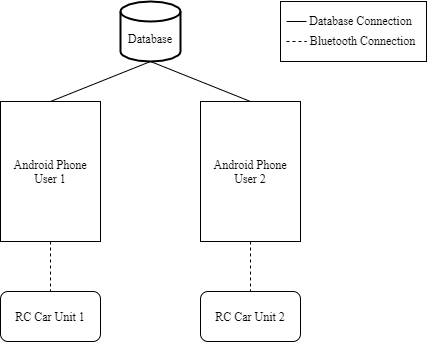
\includegraphics[width=0.8\textwidth]{Imgs/overview_of_sys.drawio.png}
    \caption{\label{fig:overview_architecture}Diagram of the Main System Architecture}
\end{figure}

\section{Hardware Architecture} \label{sec_hardware_design}

Main hardware architecture and power / harness diagram is shown in Figure \ref{fig:hardware_architecture}. 

\begin{figure}[!htbp]
    \centering
    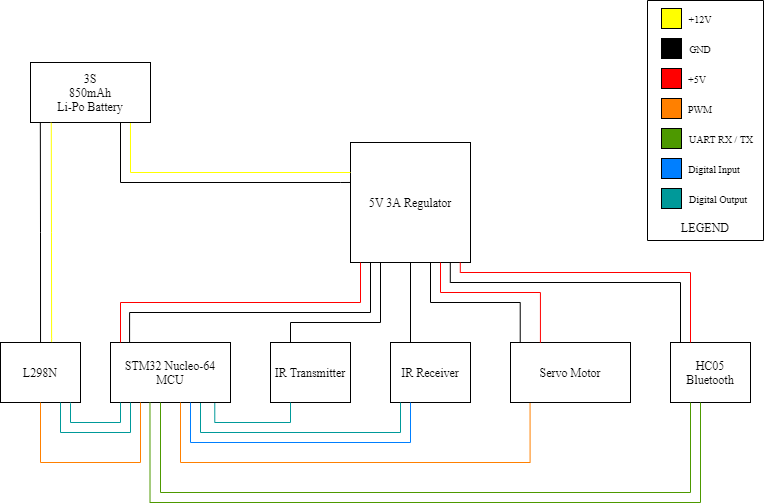
\includegraphics[width=1\textwidth]{Imgs/ana_devre_v3.png}
    \caption{\label{fig:hardware_architecture}Power / Harness Diagram of the Hardware}
\end{figure}

The system is powered from a 3S 25C 850mAh Li-Po battery. This Li-Po battery can supply a maximum current of about 20A (C x mAh). This current capacity is enough for supplying the system components. HC05 module, STM32 MCU and servo motor are powered from the regulator output. This voltage regulator is a step down voltage regulator that decreases the voltage to 5V and supplies maximum 3A current.

The L298N motor driver is controlled by 3 input pins. 2 of these three input pins are controlling the direction of the DC motor. MCU writes digital output to these pins in order to change the direction of the DC motor or completely stop the DC motor of the RC car unit. Another pin is used for controlling the DC motor speed, by applying PWM signal to enable the pin of the L298N motor driver. 

Steering of the RC car is controlled by the servo motor. This steering servo motor is powered from the voltage regulator’s 5V output and controlled from the PWM signal that is generated by the MCU of the RC car unit. 

HC05 Bluetooth\texttrademark\;module connected to the UART pins of the MCU of the RC car unit. UART baud rate has been configured at 115200. HC05 RX pin is connected to the UART TX pin of the MCU, HC05 TX pin is connected to the UART RX pin of the MCU. By this way, MCU of the RC car unit communicate over the Bluetooth\texttrademark.

The IR receiver is connected to the MCU of the RC car unit as a digital input in order to keep track of the hitting by the IR transmitter (led) coming from the opponent's RC car. The IR transmitter (led) is connected to the MCU of the RC car unit as a digital input. By this way, IR transmitter (led) can be powered with GPIO pin whenever user wants.


% Hardware Components Part Start
\subsection{STM32 MCU}
The system uses STM32 Nucleo-64 development board as a MCU of the RC car unit. STM32 Nucleo-64 development board is based on processor Arm\textregistered\;Cortex\textregistered\;M4, has 32.768 kHz crystal oscillator,  has 11 timers: up to six 16-bit, two 32-bit timers up to 100 MHz, has 512 Kbytes of flash memory and 128 Kbytes of SRAM \cite{One}. This MCU provides necessary peripherals and clock speed for the RC car unit. This board has a built-in ST link programming interface and driver which provides fast development without additional ST link devices. The implementation of the hardware and firmware is not restricted with this development board; a similar approach can be applied with any MCU that is based on Arm\textregistered\;Cortex\textregistered\;M4 family and that has sufficient number of timers, GPIOs and other essential peripherals. This development board is shown in Figure \ref{fig:nucleo64_board}.

\begin{figure}[!htbp]
    \centering
    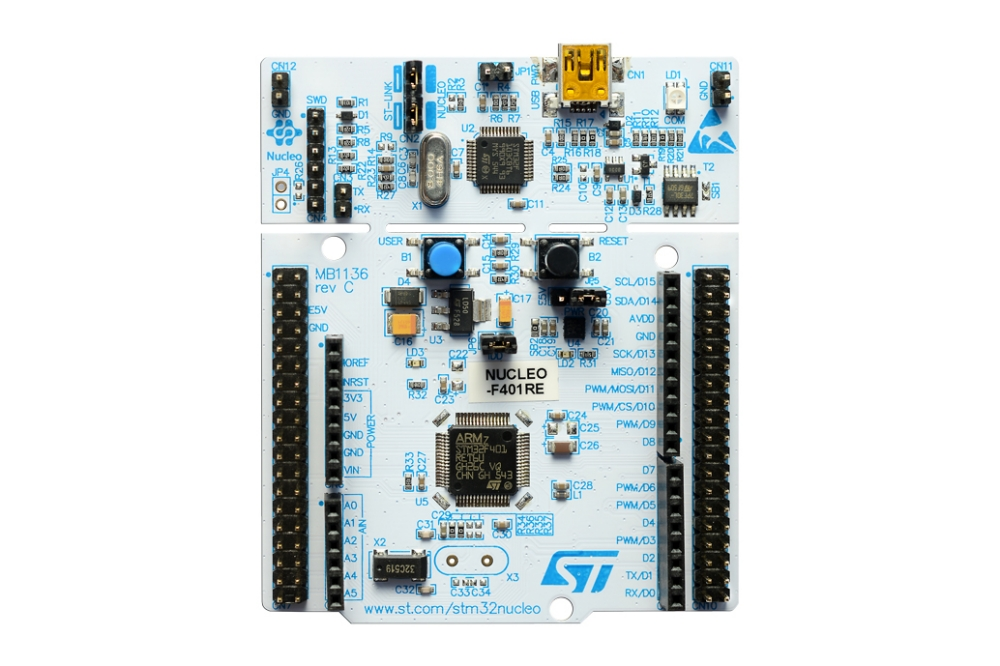
\includegraphics[width=1\textwidth]{Imgs/nucleo64.jpg}
    \caption{\label{fig:nucleo64_board}STM32 Nucleo-64 Development Board \cite{One}}
\end{figure}

\subsection{L298N DC Motor Driver} \label{sec_l298n_driver}
STMicroelectronics\texttrademark\;L298N dual full bridge DC motor driver is used for driving the DC motor of the RC car unit. It is a high voltage, high current dual full-bridge driver designed to accept standard TTL logic levels and drive inductive loads such as relays, solenoids, DC and stepping motors. Two enable inputs are provided to enable or disable the device independently of the input signals. These enable inputs accept PWM signals for driving motors with speed control. The L298N motor driver accepts 5-46V supply, provides maximum 2A DC current per channel \cite{Two}. According to these specifications and power ratings, this motor driver meets the requirements of the RC car unit. Motor driver PCB is shown in Figure \ref{fig:l298n_pcb}.

\begin{figure}[!htbp]
    \centering
    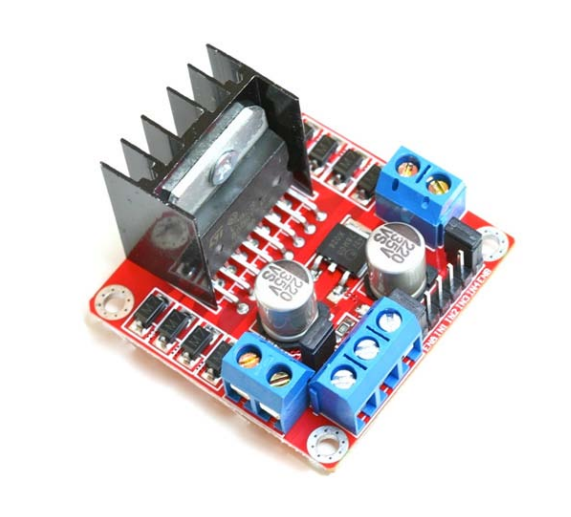
\includegraphics[width=0.6\textwidth]{Imgs/l298n.png}
    \caption{\label{fig:l298n_pcb}L298N Motor Driver PCB}
\end{figure}

\subsection{Servo Motor}
Servo motors have rapid acceleration and deceleration and provides high torques for many mechanic applications with allowing position control. High dynamic response and precision make them suitable for motion control applications and robotics. In the RC car unit, a servo motor is used for steering. Thus, precise steering control is achieving.

In this project, TowerPro\texttrademark\; MG90S servo motor is used. This servo motor works at 4.8V - 6V and has 1.8kg/cm stall torque. Maximum stall current consumption is about 1A \cite{Ref_servo_mg90s}. According to these running and power specifications, this servo motor meets the requirements of the RC car unit.

\subsection{Voltage Regulator}
LM2596 3A Step-Down Voltage Regulator is used for powering the system components which accept 5V for supply voltage. MCU, servo motor and HC05 Bluetooth\texttrademark\;module are powered from the voltage regulator output. The LM2596 series of regulators are monolithic
integrated circuits that provide all the active functions for a step-down (buck) switching regulator, capable of driving a 3-A load with excellent line and load
regulation \cite{Three}. This voltage regulator supplies enough output current for powering the 5V components in the system.

\subsection{HC05 Bluetooth Module} \label{sec_hc05_module}
The Bluetooth\texttrademark\;wireless technology is designed as a short-range networking solution for personal, portable electronic devices and embedded systems. It overcomes the limitations of line of sight and one to one communication of its possible competitor Infra-Red(IR). It operates in the 2.4 GHz Industrial, Scientific and Medical (ISM) band at a maximum data rate of 720 Kbps \cite{Bluetooth_Overview}.

In the RC car battle system, Bluetooth\texttrademark\;is used for communication between the RC car unit and the remote controller Android\texttrademark\;phone. HC05 Bluetooth\texttrademark\;module used for adding Bluetooth\texttrademark\;interface to the STM32 MCU of the system. HC05 module is Bluetooth SPP (Serial Port Protocol) module, designed for transparent wireless serial connection setup. It has an integrated antenna and programmable UART interface. Baud rate, password, name of the can be configured over this UART interface in configuration mode \cite{HC05_datasheet}. This module allows MCU to communicate with Bluetooth\texttrademark\;over the UART interface. 115200 baud rate used for UART communication with the HC05 module. This module is shown in Figure \ref{fig:hc05_module}. 

\begin{figure}[!htbp]
    \centering
    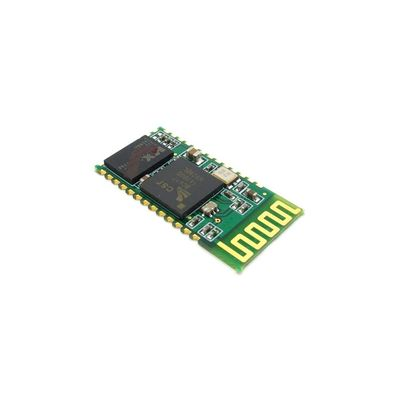
\includegraphics[width=0.5\textwidth]{Imgs/400px-HC-05.jpg}
    \caption{\label{fig:hc05_module}HC05 Bluetooth\texttrademark\; Module \cite{HC05_datasheet}}
\end{figure}

\subsection{IR Transmitter and Receiver Module}
\label{sec_ir_modules}
The RC car units simulate the shooting and hitting by IR transmitter (IR Led) and IR receiver module which. Keyestudio\texttrademark\;infrared obstacle avoidance sensor (IR-08H) used for achieving this functionality. Main purpose of this module is estimating distance by using IR led and IR receiver for obstacle avoidance applications on robotic systems. It has a pair of infrared transmitting and receiving tube. When an infrared ray launched by the transmitting tube encounters an obstacle (its reflector), the infrared ray is reflected to the receiving tube, and the indicator will light up; the signal output interface outputs a digital signal. This module works at DC 3.3V-5V voltage values. The logic level 3.3V and power consumption ratings are compatible with the MCU of the RC car unit.

The IR transmitter and receiver module has been modified for this project. A RC car unit has two of these IR modules, one for the transmitter which is on the front side of the RC car, one for receiving IR light which is on the back side of the RC car. The IR receiver part is removed from the transmitter IR module. The IR transmitter (led) part is removed from the receiver IR module.

The modified IR transmitter module of the RC car unit is shown in Figure \ref{fig:ir_transmitter}. The modified IR receiver module of the RC car unit is shown in Figure \ref{fig:ir_receiver}.

\begin{figure}[!htbp]
    \centering
    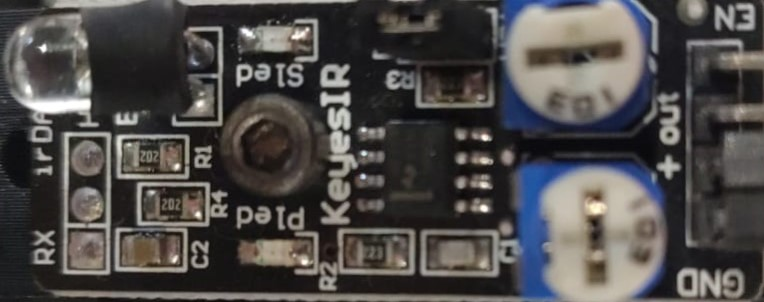
\includegraphics[width=0.50\textwidth]{Imgs/ir_transmitter.jpeg}
    \caption{\label{fig:ir_transmitter}IR Transmitter (Led) Module}
\end{figure}

\begin{figure}[!htbp]
    \centering
    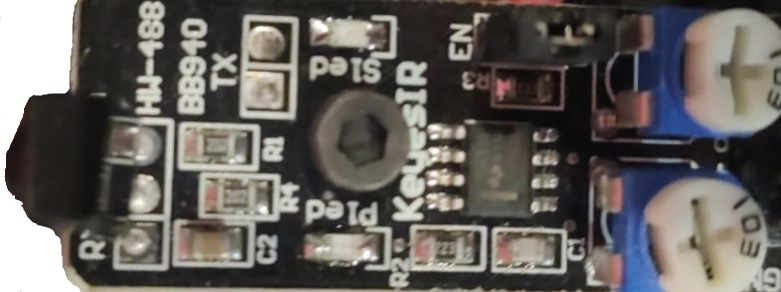
\includegraphics[width=0.55\textwidth]{Imgs/ir_receiver.jpeg}
    \caption{\label{fig:ir_receiver}IR Receiver Module}
\end{figure}

% Hardware Components Part End

\subsection{RC Car Control Unit}
\label{sec_rc_control_unit}
In this project, a custom RC car control unit has been designed on PCB. The designed and developed multi-layered PCB gathers system components under a single circuit. The PCB contains female and male headers for system components. The motivation behind designing the PCB is to avoid short circuits and poor electrical connections. The RC car control unit provides robust connection between system components and electronic modules. The designed PCB contains the following system component connections :
\begin{enumerate}
    \item Servo and DC motor male header pins.
    \item HC05 Bluetooth\texttrademark\;female header pins.
    \item STM32 MCU female header pins.
    \item Voltage regulator pad connections.
    \item L298N motor driver pad connections.
    \item Voltage divider circuit, resistor connections.
    \item Input power male header pins.
    \item Jumper for selecting the Li-Po battery ADC input with male headers.
    \item UART male header pins for debugging.
\end{enumerate}


\begin{figure}[!htbp]
    \centering
    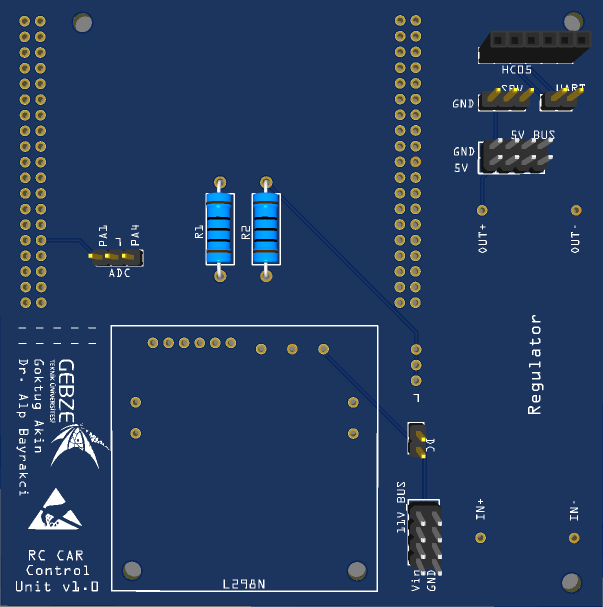
\includegraphics[width=0.6\textwidth]{Imgs/pcb.png}
    \caption{\label{fig:custom_pcb}Design view of the RC car control unit PCB}
\end{figure}

\begin{figure}[!htbp]
    \centering
    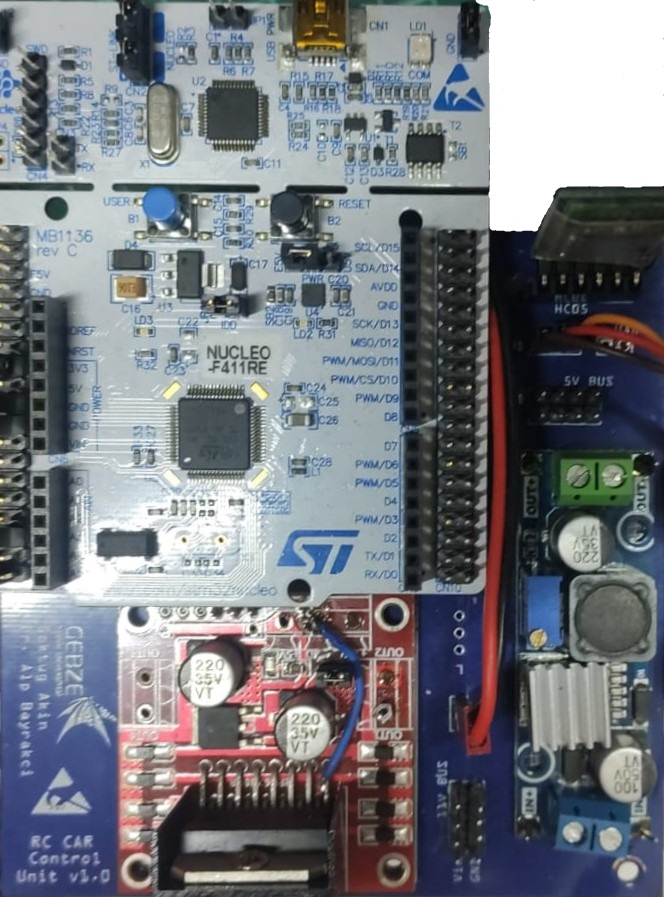
\includegraphics[width=0.6\textwidth]{Imgs/pcb_manufactured.jpeg}
    \caption{\label{fig:custom_pcb_manufactured}Manufactured RC car control unit PCB}
\end{figure}


\section{Firmware} \label{sec_firmware_design}

\subsection{Bidirectional Reliable Bluetooth Communication} \label{sec_bluetooth_comm}

Communication with the remote controller smartphone and the RC car unit is provided via Bluetooth\texttrademark.\;Hardware details of the Bluetooth\texttrademark\;are explained in the Section \ref{sec_hc05_module}. This section explains the implementation details of the bidirectional Bluetooth\texttrademark\;communication.

\subsubsection{UART RX Registers} \label{sec_receive_rc_command}

The remote controller smartphone sends RC commands to the target RC car unit at 10 HZ. HC05 module receives the incoming data from the controller smartphone, and sends this incoming data to the UART peripheral of MCU of the RC car unit. This communication runs at 115200 baud-rate.

The UART unit of the STM32 MCU generates IRQ when new data is available on the UART line. Custom ISR has been implemented for catching and handling the interrupts. The UART interrupts are used for efficient communication instead of polling methods in order to avoid consuming unnecessary cycles. The UART line is authorized in the NVIC unit of the MCU for an interrupt to occur from the UART unit of the MCU. 

To enable the read interrupts from the UART unit, RXNEIE (RX not empty interrupt enabled) bit of the CR1 (Control Register 1) has been set to 1. After this configuration, when there is new data to be read on the UART line, an interrupt will be generated from the UART unit. This control register is shown in Figure \ref{fig:uart_cr_register}. RXNEIE bit of the register highlighted in yellow.

\begin{figure}[!htbp]
    \centering
    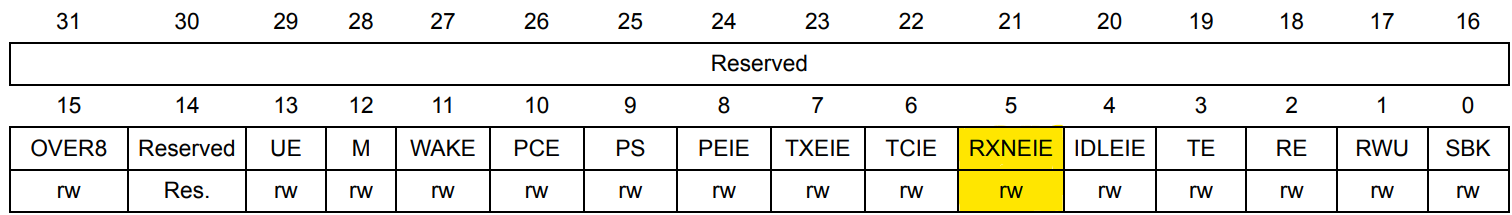
\includegraphics[width=1\textwidth]{Imgs/cr_register.png}
    \caption{\label{fig:uart_cr_register}UART Control Register 1 of the MCU (1) \cite{Ref_stm32_um}}
\end{figure}

When there is new data on the UART line, RXNE (RX not empty) bit of the status register (SR) of the UART unit is set to 1 by hardware. This bit is cleared by a read to the DR register of UART which contains the incoming data (byte). This status register is shown in Figure \ref{fig:uart_sr_register}. RXNE bit of the register highlighted in yellow.

\begin{figure}[!htbp]
    \centering
    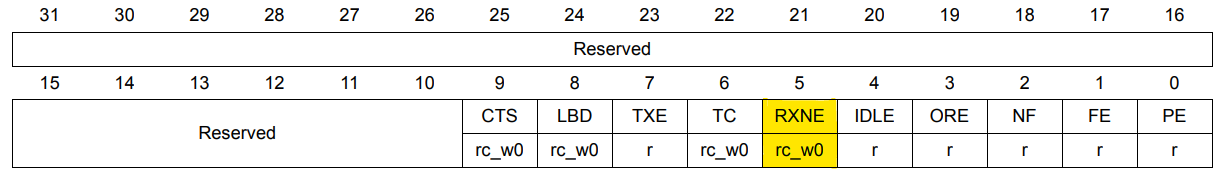
\includegraphics[width=1\textwidth]{Imgs/sr_register.png}
    \caption{\label{fig:uart_sr_register}UART Status Register of the MCU (1) \cite{Ref_stm32_um}}
\end{figure}


\subsubsection{UART TX Registers}
\label{sec_transmit_rc_info}

The RC car unit sends RC car information packets to the remote controller smartphone at 1 HZ. The MCU sends the data over the UART line, which is connected to the HC05 module. The information packet contains the version of the firmware, Li-Po battery percentage and hit counter. The controller smartphone receives these information packets in order to view them in the user interface and send the related information to the database (game server). 

The UART unit of the STM32 MCU generates IRQ when the TX sending buffer is empty for sending new data. Custom ISR is implemented for catching and handling the interrupts. When the IRQ is triggered, the data register of the UART unit is filled by the byte which is next in the ISR.

To able to enable the write available interrupts for UART unit, TXEIE (TX empty interrupt enabled) bit of the CR1 (Control Register 1) has been set to 1. After this configuration, when TX buffer of the UART unit is empty, an IRQ will be generated from the UART unit. The control register is shown in Figure \ref{fig:uart_cr_tx_register}. TXEIE bit of the register highlighted in yellow.

\begin{figure}[!htbp]
    \centering
    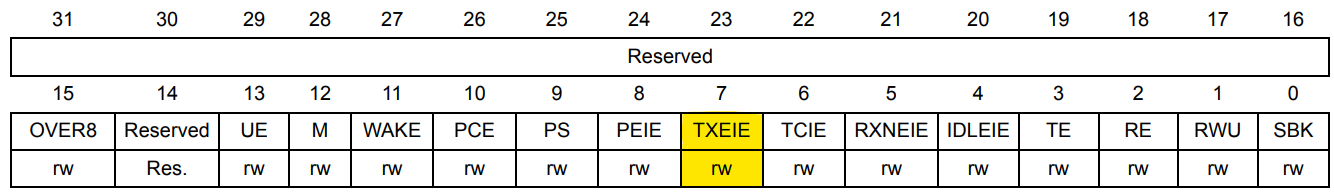
\includegraphics[width=1\textwidth]{Imgs/cr_tx_register.png}
    \caption{\label{fig:uart_cr_tx_register}UART Control Register 1 of the MCU (2) \cite{Ref_stm32_um}}
\end{figure}

When TX buffer of the UART unit is empty, TXE bit of the status register (SR) of the UART unit being set to 1 by hardware. This bit is cleared by write to the DR register of the UART unit, which contains the data (byte) to be sent to the TX buffer of the UART unit. This status register is shown in Figure \ref{fig:uart_sr_tx_register}. TXE bit of the register highlighted in yellow.

\begin{figure}[!htbp]
    \centering
    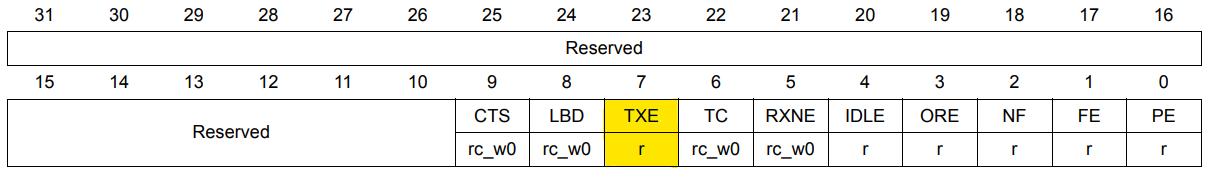
\includegraphics[width=1\textwidth]{Imgs/sr_tx_register.png}
    \caption{\label{fig:uart_sr_tx_register}UART Status Register of the MCU (2) \cite{Ref_stm32_um}}
\end{figure}


\subsubsection{UART Circular Buffer Implementation}
\label{sec_uart_circular_buff}

A circular buffer is a FIFO data structure that considers memory to be managed circularly; that is, the read/write indices loop back to 0 after it reaches the buffer length. Circular buffer has a fixed size allocated once at the system run-time. Tail and head pointers are used to indicate where to read or write to the buffer mechanism. Each time a new data sample is added (write) into the buffer, the head pointer is incremented and when the data is being read the tail pointer is incremented \cite{Ref_circ-buffer} \cite{Ref_circ_buffer_paper}. In this mechanism, producer consumer paradigm can be easily utilized over the buffer.

Circular buffer mechanism is used for bidirectional communication between the RC car unit and the remote controller smartphone. At the RC car unit side, bytes sent from the controller smartphone are being pushed into a circular buffer data structure. For transmitting data to the controller smartphone, bytes to be sent are pushed into the head position of the circular buffer. A timer generates IRQ at 1HZ, which executes sending instructions for transmitting data to the smartphone. Receiving and transmitting data procedures execute over the circular buffer.

The RC car unit firmware establishes an ISR for handling the UART interrupts for receiving and transmitting data procedures. The ISR of the UART unit is triggered when there is new data on the UART line to be read or the TX buffer of the UART line is empty to be written. This custom ISR checks the related bits of the UART registers in order to determine the source of the IRQ and manipulates the circular buffer for related operation.

The Algorithm \ref{isr_rx_algorithm} shows the pseudo code of the ISR of the UART unit.

\begin{algorithm}
\caption{ISR of UART unit}
\label{isr_rx_algorithm}
    \begin{algorithmic}
    \If{RXNE bit of the SR is 1 \textbf{AND} RXNEIE bit of the CR1 is 1}
        \State read byte from UART->DR, push into circular buffer.
        \State increment head position of the circular buffer.
    \EndIf
    \If{TXE bit of the SR is 1 \textbf{AND} TXEIE bit of the CR1 is 1}
        \If{tail position is head position}
            \State set TXEIE 0 for disabling TXE interrupts.
        \ElsIf{tail position is not head position}
            \State read byte from the circular buffer, push into USART->DR.
            \State increment tail position of the circular buffer.
        \EndIf
    \EndIf
    \end{algorithmic}
\end{algorithm}

\subsubsection{RC Command Receive State Machine}
\label{sec_rc_receive_machine}

The RC car unit firmware establishes a state machine for receiving bytes from the circular buffer, which is filled by remote controller smartphone, and evaluates these bytes for extracting the RC command packet. 10HZ RC command packet is shown in Figure \ref{fig:rc_packet}. Each field of this packet is 1 byte, totally 10 byte.

\begin{figure}[!htbp]
    \centering
    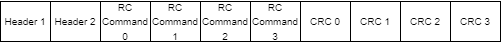
\includegraphics[width=1\textwidth]{Imgs/rc_packet.drawio.png}
    \caption{\label{fig:rc_packet}RC Command Packet Contents}
\end{figure}

The meaning of bytes in the RC command packet is shown in Table \ref{tab:rc_packet_content_table}. Each packet starts with 2 byte header for representing the starting of the RC command packet. Second start byte is reserved for the future work for representing the packet type.

\begin{table}[!htbp]
    \centering
    \caption{\label{tab:rc_packet_content_table}RC Command Packet Bytes}
    \begin{tabular}{l|r}
        Byte & Meaning \\\hline
        Header 1 & Custom start byte 1, 0x33 \\
        Header 2 & Custom start byte 2, 0x44 \\
        RC Command 0 & Steering position \\
        RC Command 1 & Throttle position \\
        RC Command 2 & Gear selection \\
        RC Command 3 & Fire, IR transmitter trigger \\
        CRC0 & 1st byte of the CRC32 value \\
        CRC1 & 2nd byte of the CRC32 value \\
        CRC2 & 3rd byte of the CRC32 value \\
        CRC3 & 4th byte of the CRC32 value \\
    \end{tabular}
\end{table}

A state machine is implemented for receiving bytes from the circular buffer and evaluating these incoming bytes according to Table \ref{tab:rc_packet_content_table}. In the main loop of the firmware, the state machine catches one byte from the circular buffer and evaluates this byte by state machine. This state machine is shown in Figure \ref{fig:rc_packet_fsm}. \\

\begin{figure}[!htbp]
    \centering
    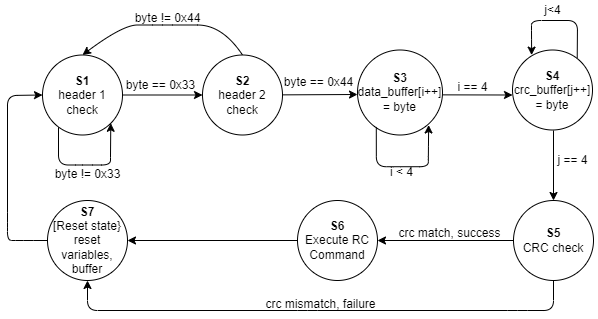
\includegraphics[width=1\textwidth]{Imgs/fsm_uart.drawio.png}
    \caption{\label{fig:rc_packet_fsm}Packet Receive State Machine}
\end{figure}

The states in the state machine is shown in Table \ref{tab:rc_fsm_states}. \\

\begin{table}[!htbp]
    \centering
    \caption{\label{tab:rc_fsm_states}State Machine States}
    \begin{tabular}{l|r}
        State & Meaning \\\hline
        S1 & Start byte 1 check, expecting byte 0x33 \\
        S2 & Start byte 2 check, expecting byte 0x44 \\
        S3 & Collecting 4 byte RC command \\
        S4 & Collecting 4 byte CRC32 \\
        S5 & CRC check with received and calculated values \\
        S6 & Evaluate RC command in case of CRC success \\
        S7 & Reset the state machine by resetting variables and buffers \\
    \end{tabular}
\end{table}

The RC car unit and the remote controller smartphone runs the packet receive state machine in order to catch the RC command and car data information packets.

\subsubsection{Cyclic Redundancy Check (CRC)}

The  Cyclic  Redundancy  Check  (CRC)  is  an  efficient  method  to  ensure  a  low  probability of undetected errors in data transmission using a checksum as a result of polynomial  division. All the characters in a message block are treated as a serial string of bits representing a binary number. This number is then divided modulo 2 by a predetermined binary number and the remainder of this division is appended to the block of characters as a cyclic redundancy check (CRC) character. The CRC is compared with the check character obtained in similar fashion at the receiving end. If they match, the data is assumed correct, otherwise incoming data / packet is discarded \cite{crc_book} \cite{crc_article}. 

The CRC method is used in the communication framework between the RC car unit and the remote controller smartphone. Each sender calculates its own CRC value and concatenates this CRC value to the sending packet. The receiver calculates the CRC value of the received packet and compares the calculated CRC value with the CRC value which is sent by the sender. In case of CRC match, packets are being evaluated / executed. 

The STM32 MCU has a built-in CRC calculation unit. This unit supports CRC32 MPEG calculation (polynomial : 0x04C11DB7). At the RC car unit side, CRC values are being calculated by hardware of the MCU since hardware calculation is efficient by comparison to software calculation. The remote controller application calculates the MPEG CRC32 by software. 

Clock cycle comparison for CRC calculation with hardware and software is shown in Table \ref{tab:crc_calc_compare} \footnote{The values in the table may differ in different models of the MCU. Exact numbers and comparison details can be found at \cite{Ref_stm32_um}.}. Input data is 256 words. Since the hardware calculation of the CRC consumes less clock cycles than the software calculation, firmware of the RC car unit utilizes hardware calculation method. \\

\begin{table}[!htbp]
    \centering
    \caption{\label{tab:crc_calc_compare}CRC Calculation Cycles}
    \begin{tabular}{l|r}
        CRC by software (system clock cycle) & CRC Peripheral (system clock cycle) \\\hline
        78094 & 1287 \\
    \end{tabular}
\end{table}


\subsection{Controlling Motors} \label{sec_controlling_motors}

\subsubsection{DC Motor Control} \label{sec_dc_motor_control}
The RC car unit uses one DC motor for accelerating the robot car. L298N motor driver is used for functional driving the dc motor. The hardware details is explained in Section \ref{sec_l298n_driver}. This driver is controlled by the MCU of the RC car control unit with 3 connections which controls the direction and speed of the motor. The MCU generates digital output for direction control on 2 GPIO pins, and PWM signal for speed control. \\

\subsubsection{Servo Motor Control} \label{sec_servo_motor_control}
The RC car unit uses one 50Hz servo motor for steering control of the robot car. The MCU generates a PWM signal for servo motor control over the GPIO pin. The MCU has an 84 MHz ABP1 timer on the related GPIO connected to the servo signal pin. This frequency needs to be decreased since the servo motor works at 50 Hz. Frequency decreasing configuration is done by changing the counter period and 16 bit prescaler parameters in order to get the target frequency 50 Hz. The timer parameters are configured as :

\begin{enumerate}
    \item Prescaler : 1680
    \item Counter Period : 1000
\end{enumerate}

According to the following formula (1), the needed 50Hz frequency is utilized from the timer, in order to generate the PWM signal for the servo motor. Same frequency division method is applied for generating DC motor PWM signals, with different division parameters.

\[50Hz = \frac{84*10^6}{1680*1000} Hz \hspace{1cm}(1)\]

All timer configurations are done with HAL on STM32 Cube MX IDE. This mechanism allows changing configurations and parameters for peripherals of the MCU during the development process.


\subsection{IR Receiver and IR Transmitter} \label{sec_ir_rx_tx}

RC car unit has IR receiver and IR transmitter module in order to hit the target car and receive the IR light from the opponent's car. The hardware details of the IR modules has explained in the Section \ref{sec_ir_modules}. 

To trigger the IR transmitter of the RC car unit, the MCU provides digital output to the GPIO pin which is connected to the IR transmitter by powering up the module. After this powering up process, the IR transmitter module powered with 3.3V, which is the logic level of the MCU.

At the receiver side, the firmware of the RC car unit establishes an ISR for catching and handling the IR receiver interrupts. At normal state, which is the state of not being hit by an opponent, the IR receiver module provides 3.3V logic output on its signal pin. The IR receiver provides a low (0V) signal on its signal pin when there is a light coming from the IR transmitter module of the opponent’s RC car unit on its receiver sensor. To be able to catch this logic level change on the GPIO pin which is connected to the output signal pin of the IR receiver module, the custom ISR keeps track of the falling edge of the incoming signal. This IRQ has been authorized on the NVIC unit of the MCU.

\subsection{Reading Li-Po Battery Voltage} \label{sec_read_lipo_voltage}

Li-Po battery voltage is being read by the MCU using ADC, over the voltage divider circuit. This voltage divider circuit is shown in Figure \ref{fig:voltage_divider_circuit}. The decreased voltage pin is connected to the MCU GPIO as an input.

\begin{figure}[!htbp]
    \centering
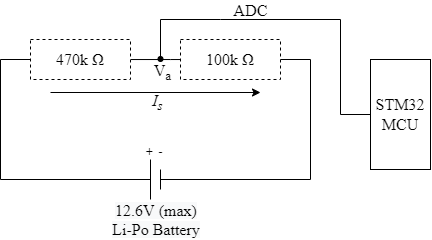
\includegraphics[width=1\textwidth]{Imgs/voltage_divider.drawio.png}
    \caption{\label{fig:voltage_divider_circuit}Voltage divider circuit diagram}
\end{figure}

The system uses 3S Li-Po battery, which provides 12.6V power at maximum charge. According to this power rating, in the voltage divider calculation, this maximum voltage value is used. Since the logic level of the STM32 MCU is 3.3V, the voltage value at the point $V_a$ must be 3.3V maximum, where $V_a$ connected to the MCU GPU as an input. According to the Ohm's Law (2), $I_s$ current is being calculated by (3).

\[V = I*R \hspace{1cm}(2)\]
\[I_s = V_L / R_e \hspace{1cm}(3)\] where $V_L$ is the Li-Po voltage and $R_e$ is the equivalent resistance. According to this formula, the current $I_s$ is calculated as :
\[I_s = 0.0221mA\hspace{1cm}(4)\]
The voltage at the point $V_a$ which is connected to the MCU, is calculated by Ohm's Law (2):
\[V_a = I_s*R_2 \hspace{1cm}(5)\] where $R_2$ is the 100k resistance. According to this formula, the maximum voltage $V_a$ is calculated as:
\[V_a = 2.21V\hspace{1cm}(6)\]
where the voltage $V_a$ meets the logic level requirements of the MCU. 

The firmware of the RC car unit establishes an ISR for reading the divided voltage of the Li-Po battery by ADC by DMA interrupts. When ADC operation is completed for reading divided Li-Po voltage, DMA interrupt is being generated and voltage value is read in the implemented ISR. After reading the voltage value, the value is pushed into a buffer with size of 10. At the 10th read, the average voltage is calculated by calculating the average value over the filled buffer. This method is called the running average method, which is useful for noise reduction.

\section{Remote Controller Application} \label{sec_remote_app}

\subsection{User Interface} \label{sec_user_interface}
The remote controller application has following user interface components for vehicle control and connection procedures:

\begin{itemize}
    \item A combo box for selecting target RC car device.
    \item Connect / Disconnect button for connecting the target RC car device.
    \item Ready button for starting / stopping online game session.
    \item Connection status label.
    \item Communication health label.
    \item Name and score of the connected RC car device.
    \item Name and score of the opponent RC car device.
    \item Slider for throttle control.
    \item Steering angle label.
    \item Application and firmware version label.
    \item Fire button for triggering the IR transmitter.
    \item Battery percentage label.
\end{itemize}

The user interface of the remote controller application is shown in Figure \ref{fig:ui_app}.

\begin{figure}[!htbp]
    \centering
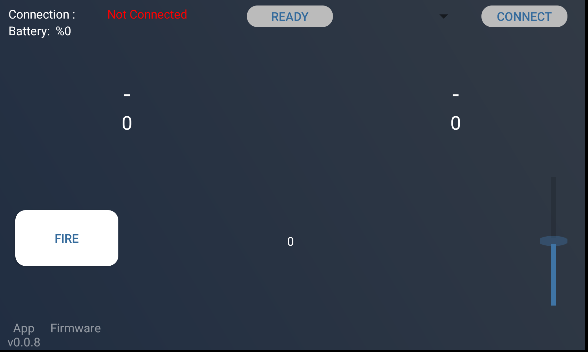
\includegraphics[width=0.9\textwidth]{Imgs/ui_app.png}
    \caption{\label{fig:ui_app}User interface of the mobile application}
\end{figure}


\subsection{RC Car Communication} \label{sec_rc_comm}
The remote controller application sends RC command packet to the target RC car unit at 10 Hz. The RC command packet contains the following information inside it :

\begin{itemize}
    \item Steering position to control the servo motor.
    \item Throttle position to control the DC motor.
    \item IR led trigger on / off.
    \item Gear selection, backward or forward.
\end{itemize}

After preparing the RC command packet according to the user interface inputs, CRC32 MPEG value is calculated in the software. The calculated CRC32 value is concatenated to the data to be sent in order to allow the RC car unit which is the receiving side to compare the calculated and sent CRC32 value.

At the receiver side, the remote controller software establishes a thread for receiving the car information packets, which contains the hit counter, battery percentage and firmware version number. This receiver thread utilizes the same state machine that is explained in Section \ref{sec_rc_receive_machine}. The content of the received car information packet is shown in Table \ref{tab:carinfo_packet_content_table}.

\begin{table}[!htbp]
    \centering
    \caption{\label{tab:carinfo_packet_content_table}Car Information Packet Bytes}
    \begin{tabular}{l|r}
        Byte & Meaning \\\hline
        Header 1 & Custom start byte 1, 0x33 \\
        Header 2 & Custom start byte 2, 0x44 \\
        Car Information Packet[0] & Major Firmware Version \\
        Car Information Packet[1] & Minor Firmware Version \\
        Car Information Packet[2] & Battery Percentage \\
        Car Information Packet[3] & Hit counter \\
        CRC0 & 1st byte of the CRC32 value \\
        CRC1 & 2nd byte of the CRC32 value \\
        CRC2 & 3rd byte of the CRC32 value \\
        CRC3 & 4th byte of the CRC32 value \\
    \end{tabular}
\end{table}


\subsection{Database Connection} \label{sec_db_connection}
Online game sessions are stored in the Google\texttrademark\;Firebase database. If a user starts an online game session over the user interface of the remote controller application, a new thread starts in order to keep the database updated. Each client connects to the game session, by adding a new entry into the game session field of the database. Data structure for storing the game session client on the database is shown in Table \ref{tab:db_fields}.

\begin{table}[!htbp]
    \centering
    \caption{\label{tab:db_fields}Game session client in database fields}
    \begin{tabular}{l|r}
        Field & Meaning \\\hline
        Fired Counter & Stores the number for fired / hit counter, caused by the opponent \\
        Timestamp & Stores for heartbeat communication between database and smartphone \\
    \end{tabular}
\end{table}

The database updater thread of the remote controller application updates the related user's timestamp and hit counter at 1Hz. This mechanism allows users to view the successful shots of him / her on the user interface. This thread also compares the opponent's timestamp with his / her timestamp in order to cancel or continue the online game session. If timestamp values of the users don't match, the remote controller application will detect this timestamp mismatch and cancel the online game session. The tree structure of the online game session in the database is designed via following structure :

\begin{itemize}
    \item RC Car Online Session
    \begin{itemize}
        \item User 1
        \begin{itemize}
            \item Timestamp
            \item Hit counter
        \end{itemize}
        \item User 2
        \begin{itemize}
            \item Timestamp
            \item Hit counter
        \end{itemize}
    \end{itemize}
\end{itemize}





\begin{comment}
% Below are comments, just for source..
\begin{algorithm}
\caption{ISR of UART line for RX interrupts}
\label{isr_rx_algorithm}
\begin{algorithmic}
\Require $n \geq 0$ % i.e. input
\Ensure $y = x^n$  % i.e. output
\State $y \gets 1$
\State $X \gets x$
\State $N \gets n$
\While{$N \neq 0$}
\If{$N$ is even}
    \State $X \gets X \times X$
    \State $N \gets \frac{N}{2}$  \Comment{This is a comment}
\ElsIf{$N$ is odd}
    \State $y \gets y \times X$
    \State $N \gets N - 1$
\EndIf
\EndWhile
\end{algorithmic}
\end{algorithm}
    Ut enim ad minima veniam, quis nostrum exercitationem ullam corporis suscipit laboriosam, nisi ut aliquid ex ea commodi consequatur? Quis autem vel eum iure reprehenderit qui in ea voluptate velit esse quam nihil molestiae consequatur, vel illum qui dolorem eum fugiat quo voluptas nulla pariatur? \ref{tab:widgetss}

    \begin{table}[!htbp]
    \centering
    \caption{\label{tab:widgetss}Comparison of percentages.}
    \begin{tabular}{c|cc|cc}
    \hline
    Mode &  \multicolumn{2}{c}{Var} & \multicolumn{2}{c}{Cum}\\ 
    \hline
    1   &  17.5 & 19.1   & 17.5  & 19.1\\
    2   &  11.8 & 12.7   & 29.3  & 31.9\\
    3   &  6.6  &  5.6   & 35.9  & 37.4\\
    \end{tabular}
    \end{table}
    
    \begin{enumerate}
    \item first,
    \item second.
    \end{enumerate}
    \dots and bullet points \dots
    \begin{itemize}
    \item one bullet,
    \item two bullets.
    \end{itemize}
    
    Let $X_1, X_2, \ldots, X_n$ be a sequence of independent and identically distributed random variables with $\text{E}[X_i] = \mu$ and $\text{Var}[X_i] = \sigma^2 < \infty$, and let
    \[S_n = \frac{X_1 + X_2 + \cdots + X_n}{n}
          = \frac{1}{n}\sum_{i}^{n} X_i\]
    denote their mean. Then as $n$ approaches infinity, the random variables $\sqrt{n}(S_n - \mu)$ converge in distribution to a normal $\mathcal{N}(0, \sigma^2)$.
    
    \begin{quote}
        At vero eos et accusamus et iusto odio dignissimos ducimus qui blanditiis praesentium voluptatum deleniti atque corrupti quos dolores et quas molestias excepturi sint occaecati cupiditate non provident, similique sunt in culpa qui officia deserunt mollitia animi, id est laborum et dolorum fuga.
    \end{quote}
\end{comment}